\chapter{Advertising: Clicks Maximization}

In this section we focus on the advertising and more precisely on the clicks maximization problem.\\
The goal of this part is to optimize the budget allocation over the three sub-campaigns in order to maximize the total number of clicks we can get.\\
In particular given the assignment~\ref{assPart2} we have designed a combinatorial bandit algorithm for addreassing this task.\\
In the following chapter we are going to:
\begin{itemize}
	\item describe the environment setup;
	\item explain the algorithm design choice;
	\item comment the obtained results.
\end{itemize}

\section{Environment}
The \textbf{Environment} returns the reward associated to each sub-campaign, by iterating over the days for the entire time horizon.\\
In our setting, it computes the optimal number of clicks knowing the real functions, one for each sub-campaign, generating  the number of clicks given a bid value \textbf{\textit{n(x)}}:\\

\begin{equation}
	n(x) = c_{M} \cdot (v_{M} - e^{-\alpha x})
\end{equation}

where:
\begin{itemize}
	\item $c_{M}$ : is the maximum number of clicks the considered sub-campaign can reach in a day;
	\item $v_{M}$ and $\alpha$ : are values associated to each sub-campaign defining the actual bidding curve.
\end{itemize}


The Environment, given the index of the bid chosen by the Learner, returns the collection of rewards associated to each sub-campaign in a completely transparant way to the learning algorithm.\\
How the learner works and its implementation will be described in the following section.



\section{Algorithm Design Choices}

This section deals with the description of the algorithm design choices we adopted and
it also contains the most relevant reference to the code.\\
In the class \textit{BiddingEnvironment.py}, which extends the class \textit{Environment.py} we have defined the actual environment we are working in, described in section before, with the definition of the bids space and the three curves \textit{n(x)}.\\
In order to find the best budget allocation over the three sub-campaigns able to maximize the total number of clicks, we have designed a combinatorial bandit algorithm.\\
In the first phase of the algorithm, we learn the model of each sub-campaign from the observation we get.
To do that in \textit{GP\_Learner.py} we have used a \textit{Gaussian process regressor}.\\
Afterward, the model of each sub-campaign is updated using those observations and the GP will reduce the uncertainty of its estimation. In this way, for each new collected sample, the function estimated by the GP approaches to the real function.\\


In order to properly used a GP regressor, we had to normalize the data. The bid space was already defined in range [0,1] and so the input variable has not to be normalized. So, we only needed to normalize the target and we have done it in the construction of the gaussian process.\\
A Gaussian proccess is completely defined by its mean and its covariance.Since we don't have any prior information we assumed to have zero mean and the covariance given by the squared exponential kernel function \textbf{k(x,x')}:
\begin{equation}
	k(x,x') = \theta^{2} e^{-\frac{(x-x')^2}{2 l^2}}
\end{equation}
where:
\begin{itemize}
	\item \textit{l} :is the \textit{lengthscale};
	\item $\theta$: is the \textit{scale factor}
\end{itemize}
The optimal value of the two hyperparameters have been found by maximiziation of the marginal likelihood during the fit proccess.
\\
\\
In the second phase of the algorithm we have used the values from the learned model to solve the problem of finding the best budget allocation to be set for the current day.\\
In the \textit{Optimizer.py} class we have implemented a modified version of the dynamic programming algorithm used for solving the knapsack problem.\\
More precisely,we have used a matrix in which each row represents the fact that at each step a new sub-campaign enters the problem, while for the columns we have discretized the whole budget in 20 possible uniformly distributed combinations of the budget allocation.\\
Each cell of the matrix contains the value of the best allocation for the considered row and column. 
The result is given by the maximization of the sum of the values provided by the best solution of the problem solved in the previous row (i.e. without considering the new entered sub-campaign) and 
the value of the new considered sub-campaign (considered singularly) s.t. the daily budget over the three sub-campaigns sums to the total daily budget.\\
Once we have filled the entire table, we have the best solution in the last row, i.e. when all the 3 sub-campaigns are considered.\\
In figure ~\ref{curve2Fig} we can see, for each sub-campaign, the real function generating the number of clicks n(x), the function learned by GP regressor and its associated uncertainty.

\begin{figure}[!htb]
	\centering
	%\captionsetup{justification=centering,margin=1cm}
	
	\begin{subfigure}[!H]{0.8\textwidth}
		\centering
		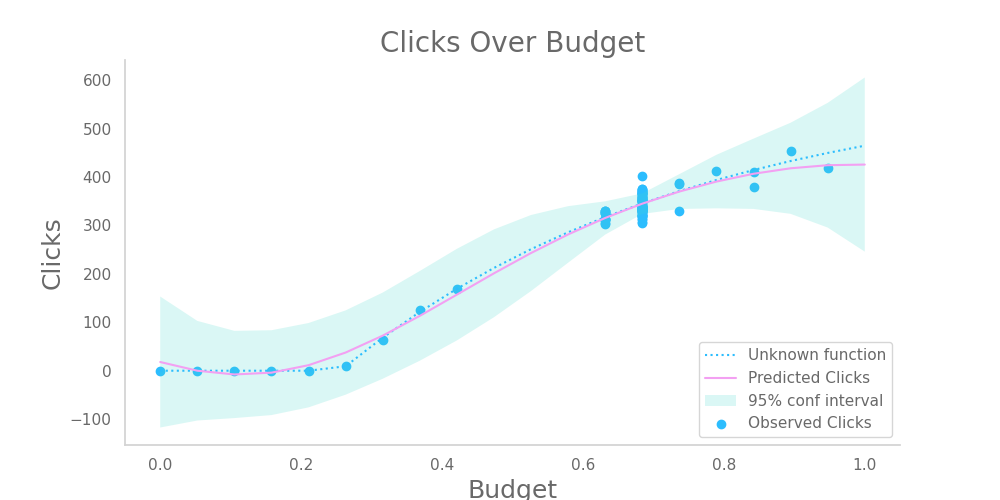
\includegraphics[width=\textwidth]{images/part2_bidding_curve_subcamaign_0.png}
	\end{subfigure}
	
	\begin{subfigure}[!H]{0.8\textwidth}
		\centering
		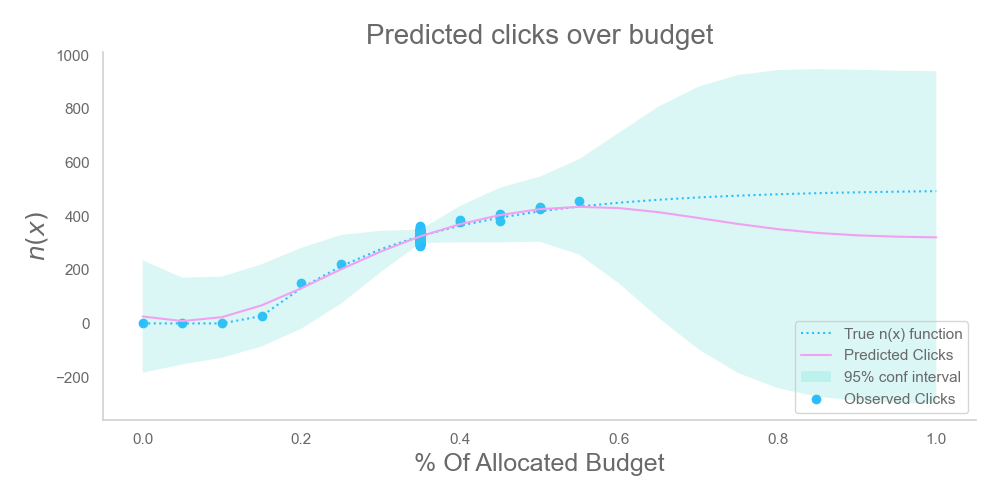
\includegraphics[width=\textwidth]{images/part2_bidding_curve_subcamaign_1.png}
	\end{subfigure}
	%\hfill
	\begin{subfigure}[!H]{0.8\textwidth}
		\centering
		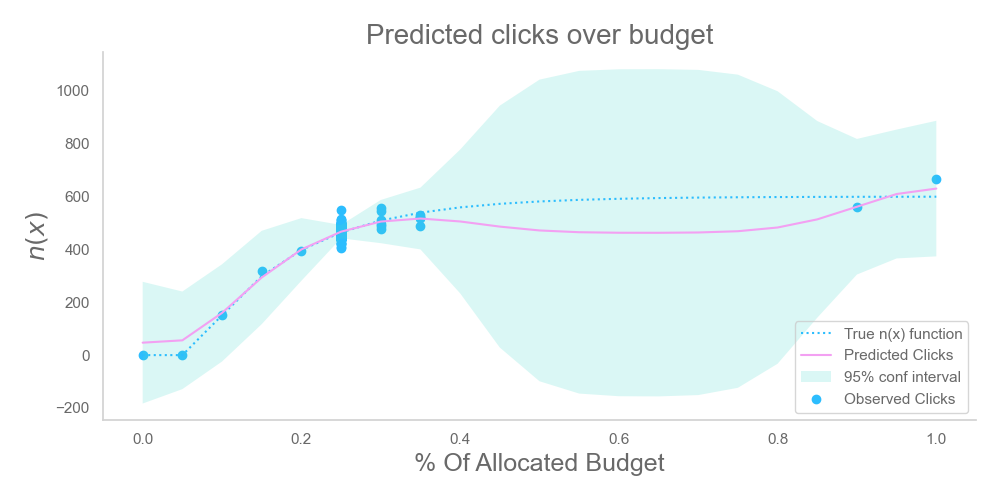
\includegraphics[width=\textwidth]{images/part2_bidding_curve_subcamaign_2.png}
	\end{subfigure}

	\caption{Functions generating the number of clicks}.
	\label{curve2Fig}
\end{figure}

\section{Performance evaluation}
In order to evaluate the performance of the implemented algorithm, we have computed the \emph{cumulative regret} as the difference between the expected reward of the \textit{Clairvoyant algorithm} and the expected reward of our combinatorial bandit algorithm.\\
In \ref{regret2Fig} the plot of the regret we obtain:
\begin{figure}[!htb]
	\centering
	%\captionsetup{justification=centering,margin=1cm}
		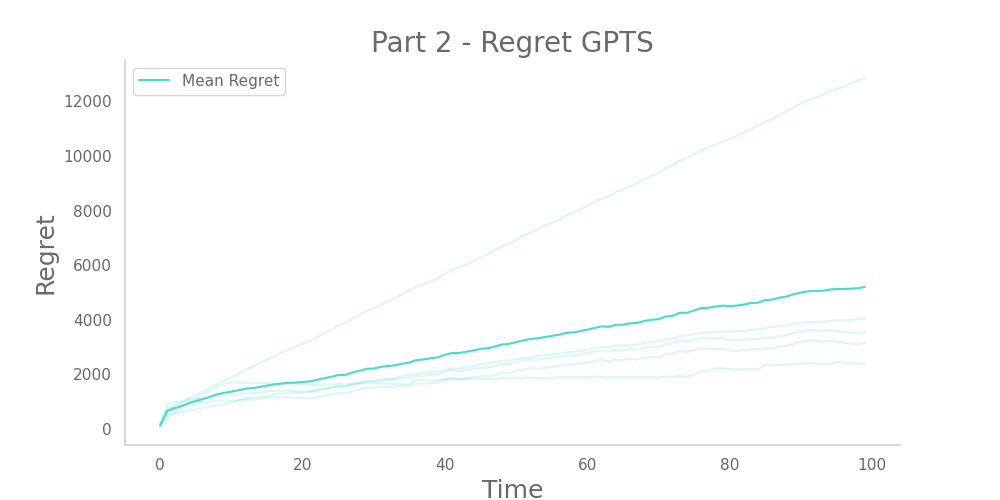
\includegraphics[width=\textwidth]{images/part2.png}
	\caption{Cumulative regret of the combinatorial bandit algorithm}.
	\label{regret2Fig}
\end{figure}


